%\title{Overleaf Memo Template}
% Using the texMemo package by Rob Oakes
\documentclass[letter,12pt]{texMemo}
\usepackage[english]{babel}
\usepackage{color, listings, graphicx, float, booktabs, multirow, outlines}
\pagenumbering{gobble}

%% Edit the header section here. To include your
%% own logo, upload a file via the files menu.
\memoto{Whom It May Concern}
\memofrom{Kyle Salitrik}
\memosubject{SQL Queries for Generating Schedules}
\memodate{\today}
%\logo{
\includegraphics[width=0.3\textwidth]{Overleaf-logo.jpg}}
\graphicspath{{./figures/}}

\definecolor{codegreen}{rgb}{0,0.6,0}
\definecolor{codegray}{rgb}{0.5,0.5,0.5}
\definecolor{codepurple}{rgb}{0.58,0,0.82}
\definecolor{backcolour}{rgb}{0.95,0.95,0.95}
 
\lstdefinestyle{mystyle}{
    backgroundcolor=\color{backcolour},   
    commentstyle=\color{codegreen},
    keywordstyle=\color{magenta},
    numberstyle=\tiny\color{codegray},
    stringstyle=\color{codepurple},
    basicstyle=\footnotesize,
    breakatwhitespace=false,         
    breaklines=true,                 
    captionpos=b,                    
    keepspaces=true,                 
    numbers=left,                    
    numbersep=5pt,                  
    showspaces=false,                
    showstringspaces=false,
    showtabs=false,                  
    tabsize=2
}
 
\lstset{style=mystyle}


\begin{document}
\maketitle

The following queries will return the desired information to create the schedule tables requested. An updated entity-relationship diagram is attached to the second page, where a shift times table was added in place of enumerations.

\section*{Department of Nurses View}
This query will return the nurse's name, the department they are assigned to, the start and end times of their shift and the day of the week. The data will be organized first by day of the week, then by the nurse's last name and finally by their first name. The start date of the week in question must be specified. 
\lstinputlisting[language=SQL]{./code/don_view.sql}

\section*{Department Manager View}
The following query will return the same columns of information for a specified week, however it will only return the information department manager assigned to that department. The data will be organized in ascending order by first department name, then the day of the week and finally the start time of the shift.
\lstinputlisting[language=SQL]{./code/dmg_view.sql}

\section*{Employee View}
Finally, the employee view will return the schedule for an employee given the employee's ID and the start date of the week. The returned information will be organized by the day of the week and then start time of the shift in case multiple shifts are scheduled.
\lstinputlisting[language=SQL]{./code/emp_view.sql}

\bigskip{}\decorativeline\bigskip{}

Sincerely,\\

\quad Kyle Salitrik

\newpage
\begin{figure}[H]
	\centering
	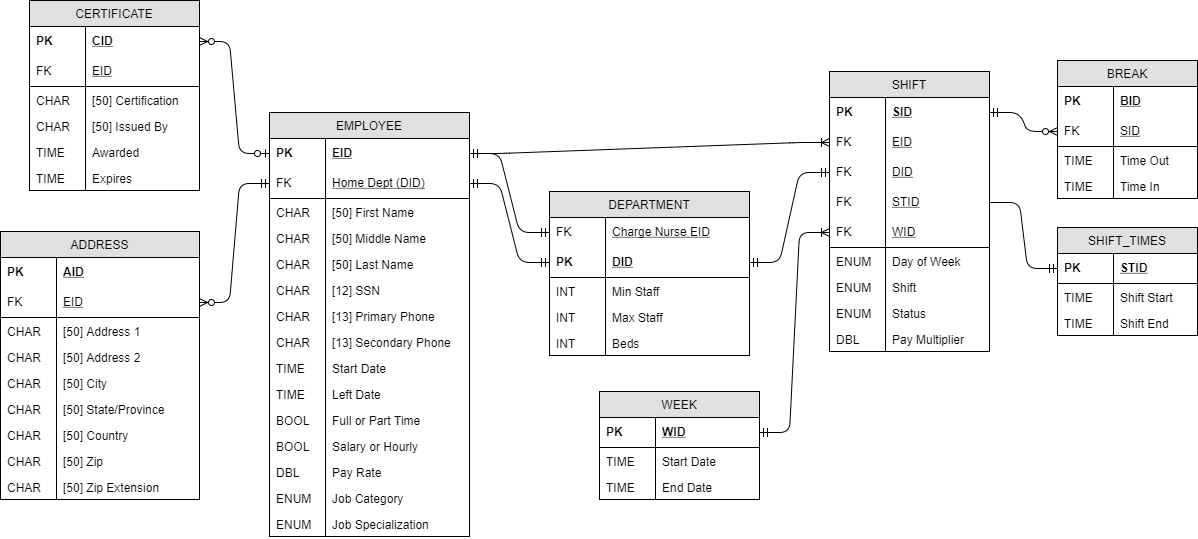
\includegraphics[angle=90, height=\textheight]{er_diag.png}
\end{figure}

\end{document}